%!TeX encoding = UTF-8
%!TeX program = xelatex
\documentclass[notheorems, aspectratio=54, tikz,border=10pt,multi]{beamer}
% aspectratio: 1610, 149, 54, 43(default), 32

\usepackage{latexsym}
\usepackage{amsmath,amssymb}
\usepackage{mathtools}
\usepackage{color,xcolor}
\usepackage{graphicx}
\usepackage{algorithm}
\usepackage{amsthm}
\DeclareMathOperator*{\argmax}{argmax} % thin space, limits underneath in displays
\usepackage{lmodern} % 解决 font warning
% \usepackage[UTF8]{ctex}
\usepackage{animate} % insert gif

\usepackage{lipsum} % To generate test text 
\usepackage{ulem} % 下划线,波浪线

\usepackage{listings} % display code on slides; don't forget [fragile] option after \begin{frame}

% ----------------------------------------------
% tikx
\usepackage{framed}
\usepackage{fancybox}
\usepackage{tikz}
\usepackage{pgf}
\usetikzlibrary{automata, calc,trees,positioning,arrows,chains,shapes.geometric,%
    decorations.pathreplacing,decorations.pathmorphing,shapes,%
    matrix,shapes.symbols, hobby}
\pgfmathsetseed{1} % To have predictable results
% Define a background layer, in which the parchment shape is drawn
\pgfdeclarelayer{background}
\pgfsetlayers{background,main}

% define styles for the normal border and the torn border
\tikzset{
  normal border/.style={orange!30!black!10, decorate, 
     decoration={random steps, segment length=2.5cm, amplitude=.7mm}},
  torn border/.style={orange!30!black!5, decorate, 
     decoration={random steps, segment length=.5cm, amplitude=1.7mm}}}

% Macro to draw the shape behind the text, when it fits completly in the
% page

\def\parchmentframe#1{
\tikz{
  \node[inner sep=2em] (A) {#1};  % Draw the text of the node
  \begin{pgfonlayer}{background}  % Draw the shape behind
  \fill[normal border] 
        (A.south east) -- (A.south west) -- 
        (A.north west) -- (A.north east) -- cycle;
  \end{pgfonlayer}}}

% Macro to draw the shape, when the text will continue in next page
\def\parchmentframetop#1{
\tikz{
  \node[inner sep=2em] (A) {#1};    % Draw the text of the node
  \begin{pgfonlayer}{background}    
  \fill[normal border]              % Draw the ``complete shape'' behind
        (A.south east) -- (A.south west) -- 
        (A.north west) -- (A.north east) -- cycle;
  \fill[torn border]                % Add the torn lower border
        ($(A.south east)-(0,.2)$) -- ($(A.south west)-(0,.2)$) -- 
        ($(A.south west)+(0,.2)$) -- ($(A.south east)+(0,.2)$) -- cycle;
  \end{pgfonlayer}}}

% Macro to draw the shape, when the text continues from previous page
\def\parchmentframebottom#1{
\tikz{
  \node[inner sep=2em] (A) {#1};   % Draw the text of the node
  \begin{pgfonlayer}{background}   
  \fill[normal border]             % Draw the ``complete shape'' behind
        (A.south east) -- (A.south west) -- 
        (A.north west) -- (A.north east) -- cycle;
  \fill[torn border]               % Add the torn upper border
        ($(A.north east)-(0,.2)$) -- ($(A.north west)-(0,.2)$) -- 
        ($(A.north west)+(0,.2)$) -- ($(A.north east)+(0,.2)$) -- cycle;
  \end{pgfonlayer}}}

% Macro to draw the shape, when both the text continues from previous page
% and it will continue in next page
\def\parchmentframemiddle#1{
\tikz{
  \node[inner sep=2em] (A) {#1};   % Draw the text of the node
  \begin{pgfonlayer}{background}   
  \fill[normal border]             % Draw the ``complete shape'' behind
        (A.south east) -- (A.south west) -- 
        (A.north west) -- (A.north east) -- cycle;
  \fill[torn border]               % Add the torn lower border
        ($(A.south east)-(0,.2)$) -- ($(A.south west)-(0,.2)$) -- 
        ($(A.south west)+(0,.2)$) -- ($(A.south east)+(0,.2)$) -- cycle;
  \fill[torn border]               % Add the torn upper border
        ($(A.north east)-(0,.2)$) -- ($(A.north west)-(0,.2)$) -- 
        ($(A.north west)+(0,.2)$) -- ($(A.north east)+(0,.2)$) -- cycle;
  \end{pgfonlayer}}}

% Define the environment which puts the frame
% In this case, the environment also accepts an argument with an optional
% title (which defaults to ``Example'', which is typeset in a box overlaid
% on the top border
\newenvironment{parchment}[1][Example]{%
  \def\FrameCommand{\parchmentframe}%
  \def\FirstFrameCommand{\parchmentframetop}%
  \def\LastFrameCommand{\parchmentframebottom}%
  \def\MidFrameCommand{\parchmentframemiddle}%
  \vskip\baselineskip
  \MakeFramed {\FrameRestore}
  \noindent\tikz\node[inner sep=1ex, draw=black!20,fill=white, 
          anchor=west, overlay] at (0em, 2em) {\sffamily#1};\par}%
{\endMakeFramed}

% ----------------------------------------------

\mode<presentation>{
    \usetheme{CambridgeUS}
    % Boadilla CambridgeUS
    % default Antibes Berlin Copenhagen
    % Madrid Montpelier Ilmenau Malmoe
    % Berkeley Singapore Warsaw
    \usecolortheme{beaver}
    % beetle, beaver, orchid, whale, dolphin
    \useoutertheme{infolines}
    % infolines miniframes shadow sidebar smoothbars smoothtree split tree
    \useinnertheme{circles}
    % circles, rectanges, rounded, inmargin
}
% 设置 block 颜色
\setbeamercolor{block title}{bg=red!30,fg=white}

\newcommand{\reditem}[1]{\setbeamercolor{item}{fg=red}\item #1}

% 缩放公式大小
\newcommand*{\Scale}[2][4]{\scalebox{#1}{\ensuremath{#2}}}

% 解决 font warning
\renewcommand\textbullet{\ensuremath{\bullet}}

% ---------------------------------------------------------------------
% flow chart
\tikzset{
    >=stealth',
    punktchain/.style={
        rectangle, 
        rounded corners, 
        % fill=black!10,
        draw=white, very thick,
        text width=6em,
        minimum height=2em, 
        text centered, 
        on chain
    },
    largepunktchain/.style={
        rectangle,
        rounded corners,
        draw=white, very thick,
        text width=10em,
        minimum height=2em,
        on chain
    },
    line/.style={draw, thick, <-},
    element/.style={
        tape,
        top color=white,
        bottom color=blue!50!black!60!,
        minimum width=6em,
        draw=blue!40!black!90, very thick,
        text width=6em, 
        minimum height=2em, 
        text centered, 
        on chain
    },
    every join/.style={->, thick,shorten >=1pt},
    decoration={brace},
    tuborg/.style={decorate},
    tubnode/.style={midway, right=2pt},
    font={\fontsize{10pt}{12}\selectfont},
}
% ---------------------------------------------------------------------

% code setting
\lstset{
    language=C++,
    basicstyle=\ttfamily\footnotesize,
    keywordstyle=\color{red},
    breaklines=true,
    xleftmargin=2em,
    numbers=left,
    numberstyle=\color[RGB]{222,155,81},
    frame=leftline,
    tabsize=4,
    breakatwhitespace=false,
    showspaces=false,               
    showstringspaces=false,
    showtabs=false,
    morekeywords={Str, Num, List},
}
% ---------------------------------------------------------------------

%% preamble
\title{Statistical Modeling}
% \subtitle{The subtitle}
\author{Dihui Lai}
\institute[WUSTL]{dlai@wustl.edu}


% -------------------------------------------------------------

\begin{document}

%% title frame
\begin{frame}
    \titlepage
\end{frame}


\begin{frame}
CONTENT
\begin{itemize}
\item Loss Function
\item Variable Selection
\item Feature Engineer
\item Overfitting \& Corss-validation
\end{itemize} 
\end{frame}


%% normal frame
\section{Loss Function}

\begin{frame}
\frametitle{Building Statistical Models: Likelihood/Loss Function}
\begin{itemize}
\item We are planting some seeds in your garden. What kind of distribution shall we use if we want to know the number of seeds germinate depending on the amount of water and fertilizer (Poisson/Logistic).
\item You were asked to develop an algorithm that makes predictions about the future sale prices of homes (Gaussian).
\item A researcher is interested in how variables, such as GRE (Graduate Record Exam scores), GPA (grade point average) and prestige of the undergraduate institution, effect admission into graduate school (Logistic).
\item A health-related researcher is studying the number of hospital visits in past 12 months by senior citizens in a community based on the characteristics of the individuals and the types of health plans under which each one is covered (Poisson).
\end{itemize}

\end{frame}


\begin{frame}
\frametitle{How to select a Likelihood/Loss function?}
\begin{itemize}
\item Determine the distribution of the target variable e.g. histogram
\item Make a guess and verify
\item Use the likelihood/loss function that is given to you (by your boss, a client or a stakeholder)
\end{itemize}
\end{frame}
\begin{frame}

\frametitle{How to select a Likelihood/Loss function ... More...?}
\begin{itemize}
\item MNIST handwriting data set classification (soft-max)
\item Speech recognition/Optical character recognition (connectionist temporal classification)
\end{itemize}

\end{frame}
\section{Variable Selection}

\begin{frame}
\frametitle{Goodness of Fit}

The metrics to measure the goodness of a model fitting
\begin{itemize}
\item Liklihood function$$\ell=\sum_{j} \left[y^j\theta^j-b(\theta^j)\right]$$

\item Deviance $$D=\ell_{max}-\ell(\theta (\hat{\beta}))$$ where $ell_{max}$ is the log likelihood of the saturated model.

\item AIC: $${\displaystyle \mathrm {AIC} \,=\,2k-2\ln({{\ell}})}$$
Here, k is the number of estimated parameters in the model. Besides maximizing the likelihood, AIC also penalize the complexity of a model.

\end{itemize}
\end{frame}

\begin{frame}
\frametitle{Goodness of Fit: Continued}
\begin{itemize}
\item BIC: $${\displaystyle \mathrm {BIC} \,=\,\log(n)k-2\ln({{\ell}})}$$
Here, n is the number of data points. Similar to AIC but penalize more on the model compelxity weighted by the amount of data.
\end{itemize}
\end{frame}

\begin{frame}
\frametitle{Variable Selection}
\begin{itemize}
\item Determine the contribution of a variable to the following metrics: Likelihood/Loss function, Deviance, AIC and BIC
\item Beware of target leak.
\item Consider the context of application. Is the variable available in application scenario?
\item Does it make intuitive sense?
\item Variable's statistic significance, p-value (reject the variable if p-value is above certain threshold e.g. $>0.05$, $>0.01$ etc.).
\end{itemize}
\end{frame}

\section{Feature Engineer}
\begin{frame}
\frametitle{Feature Engineer}
\begin{itemize}
\item Categorical variables
      \begin{itemize}
        \item[-] Regrouping
        \item[-] Converting to numeric version
      \end{itemize}
\item Numeric variables
      \begin{itemize}
        \item[-] Function transformation: polynomial, spline, power function, exponential, log etc.
      \end{itemize}
      
\item Variable interactions
\item Features from sub-models
\end{itemize}
\end{frame}

\section{Overfitting \& Cross-Validation}

\begin{frame}
\frametitle{Overfitting \& Cross validation}
\begin{itemize}
\item When a model becomes over-complex, it starts to fit noises rather than the true pattern
\item Training data v.s. validation data: one way to prevent overfitting is to split data into training set and validation set. If the model peforms significantly worse in the validationd data, it shows a sign of overfitting. 
\item Cross validation.
\end{itemize}
\end{frame}
\begin{center}
    
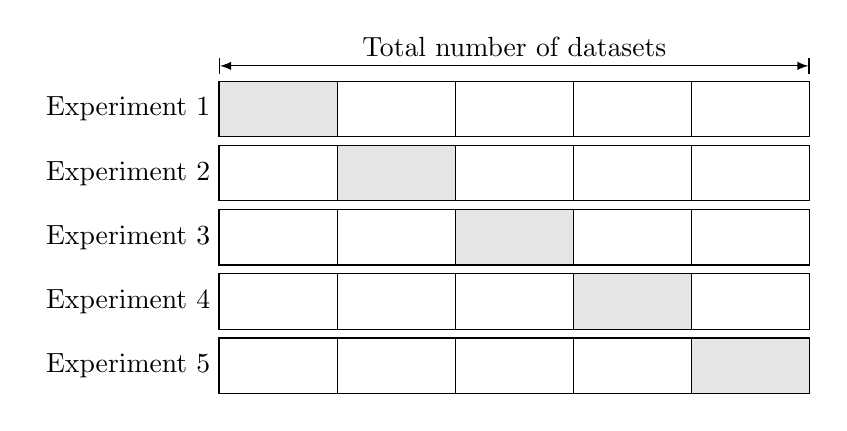
\begin{tikzpicture}
    \matrix (M) [matrix of nodes,
        nodes={minimum height = 7mm, minimum width = 1.5cm, outer sep=0, anchor=center, draw},
        column 1/.style={nodes={draw=none}, minimum width = 4cm},
        row sep=1mm, column sep=-\pgflinewidth, nodes in empty cells,
        e/.style={fill=black!10}
      ]
      {
        Experiment 1 & |[e]| & & & & \\
        Experiment 2 & & |[e]| & & & \\
        Experiment 3 & & & |[e]| & & \\
        Experiment 4 & & & & |[e]| & \\
        Experiment 5 & & & & & |[e]| \\
      };
      \draw (M-1-2.north west) ++(0,2mm) coordinate (LT) edge[|<->|, >= latex] node[above]{Total number of datasets} (LT-|M-1-6.north east);

\end{tikzpicture}

\end{center}





\end{document}
